%%%% rl_pitch_coach.tex
%%
%% Uruti RL Pitch Coach: A Deep Q-Network Approach to Automated
%% Startup Pitch Coaching via Multimodal Reinforcement Learning
%% Submitted to Deep Learning Indaba
%% Formatted for IJCAI--ECAI 2026

\typeout{Uruti RL Pitch Coach -- Deep Learning Indaba}

\documentclass{article}
\pdfpagewidth=8.5in
\pdfpageheight=11in

\usepackage{ijcai26}

% Core packages
\usepackage{times}
\usepackage{soul}
\usepackage{url}
\usepackage[hidelinks]{hyperref}
\usepackage[utf8]{inputenc}
\usepackage[small]{caption}
\usepackage[font=small,skip=4pt]{subcaption}
\usepackage{graphicx}
\usepackage{amsmath}
\usepackage{amsthm}
\usepackage{amssymb}
\usepackage{booktabs}
\usepackage{algorithm}
\usepackage{algorithmic}
\usepackage{multirow}
\usepackage{placeins}
\usepackage{xcolor}
\usepackage{tikz}
\usepackage{pgfplots}
\pgfplotsset{compat=1.17}
\usetikzlibrary{arrows.meta, positioning, shapes.geometric, fit, backgrounds}

\usepackage[authoryear,round]{natbib}

\makeatletter
\renewcommand\paragraph{\@startsection{paragraph}{4}{\z@}%
  {-4pt plus -2pt minus -1pt}%
  {0.5ex plus 0.2ex}%
  {\normalsize\bf}}
\makeatother

\urlstyle{same}
\newtheorem{definition}{Definition}

\pdfinfo{
/TemplateVersion (IJCAI.2026.0)
}

%% -----------------------------------------------------------------------
%%  Title and Authors
%% -----------------------------------------------------------------------

\title{A Deep Q-Network Pitch Coach for Startup Founders:\\
       MDP Formulation, Hyperparameter Tuning, and\\
       Multimodal Reinforcement Learning on CMU-MOSEI}

\author{
    Anonymous Submission
}

\begin{document}

\maketitle

%% -----------------------------------------------------------------------
%%  Abstract
%% -----------------------------------------------------------------------

\begin{abstract}
Effective pitch delivery is a critical yet under-coached skill for startup
founders in resource-constrained environments.
We present \textbf{PitchEnv-v1}, a custom OpenAI Gymnasium environment that
formalises startup pitch coaching as a Markov Decision Process (MDP) grounded
in the CMU-MOSEI multimodal corpus.
The environment exposes a 12-dimensional continuous state space capturing
nine pitch-quality features (eye contact, smile rate, head stability,
pause ratio, speech rate, sentiment, clarity, vocal energy, filler words)
alongside three session-state scalars.
A six-action discrete action space encodes coach interventions, and a
multi-component reward function incentivises continuous improvement,
consistency, time management, and elite delivery.
A supervised MLP reward model ($R^2 = 0.9512$) maps raw multimodal features
to coaching scores. We train four RL algorithms (DQN, PPO, TRPO, A2C) for
500{,}000 timesteps; DQN achieves the best mean final score
(\textbf{57.79/100}) and the highest success rate (\textbf{12.4\%} of
episodes reaching the elite threshold of 85/100), with DQN coaching
producing a \textbf{+12.4-point} improvement in a user acceptance trial
across eight founders.
Hyperparameter ablations identify $\gamma = 0.99$,
\textit{exploration\_fraction} = 0.6, and \textit{batch\_size} = 128 as
optimal for this environment.
\end{abstract}

%% -----------------------------------------------------------------------
%%  1. Introduction
%% -----------------------------------------------------------------------

\FloatBarrier
\section{Introduction}

Pitch delivery is one of the highest-leverage skills for a startup founder:
a compelling three-minute pitch can unlock access to accelerators, angel
investors, and grant programmes that would otherwise remain out of reach.
Yet structured, personalised pitch coaching remains a scarce resource
in Sub-Saharan Africa, where physical accelerators accept fewer than 3\%
of applicants~\citep{gem2022africa}.

Reinforcement learning (RL) offers a principled framework for automated
coaching: an agent observes a multi-dimensional behavioural state,
selects a targeted intervention, and receives a reward signal calibrated
to pedagogical outcomes.
Prior work has applied RL to educational settings~\citep{mnih2015,schulman2017},
but no prior system has grounded this formalism in multimodal
pitch-performance features from real presentation recordings.

This paper makes four primary contributions.
First, we introduce \textbf{PitchEnv-v1}, a reproducible OpenAI Gymnasium
environment that models pitch coaching as a fully-specified MDP, including a
precise definition of the state space, action space, transition dynamics, and
reward function.
Second, we design and train a \textbf{Reward MLP} that maps nine CMU-MOSEI
pitch features~\citep{zadeh2018} to a coaching score, achieving $R^2 = 0.9512$
on the held-out validation set.
Third, we conduct a \textbf{hyperparameter ablation} via a systematic grid
search over the four most impactful DQN hyperparameters ($\gamma$,
$\varepsilon$-schedule, batch size, episode length), identifying the
optimal configuration for this coaching domain.
Fourth, we provide a full \textbf{empirical evaluation} comprising reward
convergence curves, per-algorithm success counts, and a user acceptance trial
(UAT) with eight Rwandan founders showing a mean improvement of $+12.4$ points.

%% -----------------------------------------------------------------------
%%  2. Background and Related Work
%% -----------------------------------------------------------------------

\FloatBarrier
\section{Background and Related Work}

\FloatBarrier
\subsection{Deep Reinforcement Learning}

Deep Q-Networks~\citep{mnih2015} combine Q-learning with a neural function
approximator to handle high-dimensional state spaces. The agent maintains
a replay buffer $\mathcal{D}$ of transitions $(s_t, a_t, r_t, s_{t+1})$
and minimises the temporal-difference loss:
\begin{equation}
\mathcal{L}(\theta) = \mathbb{E}_{(s,a,r,s') \sim \mathcal{D}}
  \!\left[\!\left(r + \gamma \max_{a'} Q_{\hat\theta}(s',a') - Q_\theta(s,a)\right)^{\!2}\right]
\label{eq:dqn_loss}
\end{equation}
where $Q_{\hat\theta}$ is a periodically-updated target network that prevents
oscillation. Proximal Policy Optimisation~\citep{schulman2017} constrains
policy updates via a clipped surrogate objective, trading off sample
efficiency for stability. Both algorithms are benchmarked in
Section~\ref{sec:results} alongside TRPO and A2C.

In PitchEnv-v1, Deep RL is applied directly to the pitch coaching problem.
The environment's 12-dimensional state encodes the founder's current
acoustic, visual, and linguistic performance metrics; the agent selects
one of six targeted coaching interventions at each 15-second step; and the
reward signal is computed by a pre-trained MLP that translates those
behavioural signals into a holistic coaching score. This formulation
means the DQN policy learns \emph{which aspect of the pitch to coach next}
given the founder's current state --- a decision that is too context-sensitive
for rule-based heuristics and too high-frequency for human coaches to handle
in real time. The DQN architecture is chosen over continuous-action methods
because the coaching interventions are inherently discrete (e.g.~``slow down
pace'' or ``improve eye contact''), and the compact action space of six
allows efficient Q-value estimation with a two-hidden-layer MLP.

\FloatBarrier
\subsection{Multimodal Coaching and CMU-MOSEI}

The CMU-MOSEI corpus~\citep{zadeh2018} provides 23{,}453 annotated
sentence-level video segments from YouTube, each paired with acoustic
features, visual facial action units, and sentiment labels in a unified
multimodal alignment framework. Its richness of modalities makes it the
canonical benchmark for audio-visual coaching tasks: acoustic energy,
pause ratios, and facial stability are all directly observable signals of
presentation quality. For PitchEnv-v1, we extract nine pitch-relevant
feature channels from a 1{,}000-segment aligned subset
(Section~\ref{sec:features}), treating CMU-MOSEI annotations as a
proxy for expert coaching scores.

\FloatBarrier
\subsection{RLHF and Reward Engineering for Coaching}

\citet{ouyang2022instructgpt} demonstrated that reinforcement learning
from human feedback (RLHF) produces models whose outputs are more aligned
with expert intent: a learned reward model replaces brittle
handcrafted objectives and adapts to nuanced human preference.
\citet{wang2025rlhf} extended this paradigm specifically to speech and
language tasks, showing that preference-based feedback yields measurably
more helpful and grammatically coherent outputs, while simultaneously
warning that insufficiently constrained reward functions invite
\emph{reward hacking} -- artificially inflating proxy metrics without
genuine skill improvement. PitchEnv-v1 addresses this risk directly by
pairing the MLP reward model (Section~\ref{sec:reward_mlp}) with an
explicit pacing penalty and a maintenance bonus, making it costly for
the agent to game a single feature dimension at the expense of others.

\FloatBarrier
\subsection{AI-Assisted Public Speaking and Pitch Coaching}

\citet{fourati2025public} surveyed domain experts on AI-augmented
public-speaking training, concluding that AI excels at delivering
consistent, repeatable feedback on objectively measurable dimensions
(eye contact, speech rate, filler-word ratio) but falls short on
high-order qualities such as narrative coherence and charisma.
Their participants recommended deploying AI to automate repetitive
pre-acceleration practice, freeing human coaches for strategic
guidance -- precisely the role PitchEnv-v1 is designed to fill.
Complementarily, \citet{nagaram2024rlaif} introduced reinforcement
learning with AI feedback (RLAIF) for emotional expression in
text-to-speech synthesis, demonstrating that an AI teacher model can
generate nuanced preference labels at a fraction of the cost of human
annotation. This motivates PitchEnv-v1's use of a data-driven MLP
reward proxy in place of costly expert labelling.

\FloatBarrier
\subsection{AI Coaching Effectiveness in the African Context}

\citet{gem2022africa} documented that fewer than 12\,\% of Sub-Saharan
African entrepreneurs access structured mentorship, a scarcity that
systematically depresses startup survival rates.
\citet{otis2024ai} investigated this gap through a large-scale field
experiment with 640 Kenyan entrepreneurs, finding that high-performing
founders improved by over 15\,\% when given AI coaching tools, while
low-performers deteriorated by 8\,\% due to plausible but contextually
flawed advice from generic models. This asymmetry motivates
PitchEnv-v1's contextualised reward: rather than routing all founders
through a one-size-fits-all chatbot, the environment adapts action
selection to each founder's current pitch-feature profile, reducing
the risk of misdirected feedback for weaker participants.
\citet{rambe2026africa} reinforce this argument, noting that
infrastructural shortfalls and talent scarcity in Sub-Saharan Africa
necessitate AI tools that are both contextually grounded and
computationally lightweight -- design requirements that shaped every
architectural decision in PitchEnv-v1.

%% -----------------------------------------------------------------------
%%  3. The PitchEnv-v1 Environment
%% -----------------------------------------------------------------------

\FloatBarrier
\section{The PitchEnv-v1 Environment}
\label{sec:env}

We formalise pitch coaching as a Markov Decision Process
$\mathcal{M} = (\mathcal{S},\, \mathcal{A},\, \mathcal{T},\, \mathcal{R},\, \gamma)$,
implemented as a custom environment conforming to the OpenAI Gymnasium API.

\FloatBarrier
\subsection{Environment Overview}

A single \textbf{episode} represents one complete pitch presentation.
The presentation is divided into $L = 20$ discrete \textbf{steps}
(one step $\approx$ 15 seconds of real-time speech), corresponding to
a 5-minute startup pitch.
At each step the environment returns the current 12-dimensional observation
vector $s_t$, accepts a discrete coaching action $a_t \in \{0,\ldots,5\}$,
and applies the coaching intervention by perturbing the relevant feature
channels stochastically to model imperfect uptake by the founder.
It then queries the reward MLP to compute the updated coaching score
$\text{score}_{t+1}$, and returns reward $r_t$ (Eq.~\ref{eq:reward}) together
with the updated observation $s_{t+1}$.
An episode terminates after $L = 20$ steps. The terminal bonus
(Eq.~\ref{eq:terminal_bonus}) is applied if
$\text{score}_{20} \geq 85$~--- the ``expert delivery'' threshold.

\FloatBarrier
\subsection{State Space}
\label{sec:states}

\begin{definition}[State Space]
The state space is $\mathcal{S} \subseteq [0,1]^{12}$, a 12-dimensional
continuous observation vector partitioned into two groups:
\end{definition}

\paragraph{Group 1 — Pitch-Performance Features ($\mathbf{s}^{(9)}$).}
Nine normalised scalar features extracted from the CMU-MOSEI multimodal
corpus (Table~\ref{tab:state_space}). Each feature is min-max normalised
to $[0, 1]$ across the training set.

\paragraph{Group 2 — Session-Context Features ($\mathbf{s}^{(3)}$).}
Three scalar signals tracking the progression of the current episode:
(1)~\texttt{slide\_index} $\in \{0,\ldots,9\}$ normalised by 9,
(2)~\texttt{time\_remaining} $\in [0, 1]$ fraction of episode budget left,
(3)~\texttt{time\_on\_slide} $\in [0, 1]$ fraction of allocated slide
time consumed so far.

\begin{table}[htbp]
\centering
\caption{Pitch-performance state features (Group 1 of 12).
Each is a real value in $[0, 1]$ drawn from the CMU-MOSEI corpus
plus Gaussian noise $\mathcal{N}(0, 0.05)$ at each step.}
\label{tab:state_space}
\small
\begin{tabular}{lll}
\toprule
\textbf{Index} & \textbf{Feature} & \textbf{Description} \\
\midrule
$s_0$ & \texttt{eye\_contact}   & Fraction of time gaze directed at audience \\
$s_1$ & \texttt{smile\_rate}    & Proportion of frames with detectable smile \\
$s_2$ & \texttt{head\_stability}& Inverse of head-motion variance (AU normalised) \\
$s_3$ & \texttt{pause\_ratio}   & Fraction of speech time spent in pauses \\
$s_4$ & \texttt{speech\_rate}   & Syllables per second, normalised to $[0,1]$ \\
$s_5$ & \texttt{sentiment\_score}& Multimodal sentiment (CMU-MOSEI label) \\
$s_6$ & \texttt{clarity\_score} & LM-based lexical clarity (0 = unclear, 1 = clear) \\
$s_7$ & \texttt{vocal\_energy}  & Normalised RMS amplitude of audio signal \\
$s_8$ & \texttt{filler\_words}  & Fraction of words that are fillers (um, uh, like) \\
\midrule
$s_9$ & \texttt{slide\_index}   & Current slide number / 9 \\
$s_{10}$ & \texttt{time\_remaining} & Remaining episode budget / $L$ \\
$s_{11}$ & \texttt{time\_on\_slide} & Time on current slide / allocated slide time \\
\bottomrule
\end{tabular}
\end{table}

\FloatBarrier
\subsection{Action Space}
\label{sec:actions}

\begin{definition}[Action Space]
The action space is $\mathcal{A} = \{0,1,2,3,4,5\}$ (Discrete(6)).
Each action encodes a specific coaching intervention delivered to the
presenter.
\end{definition}

\begin{table}[htbp]
\centering
\caption{Coaching action definitions and their primary effect on the
state vector. Feature deltas are sampled as
$\delta \sim \mathcal{U}(0.05, 0.15)$ to model imperfect uptake.}
\label{tab:actions}
\small
\begin{tabular}{lll}
\toprule
\textbf{Action} & \textbf{Intervention} & \textbf{Primary Feature Effect} \\
\midrule
0 & Increase Energy     & $\uparrow s_7$ (vocal energy) \\
1 & Improve Eye Contact & $\uparrow s_0$ (eye contact), $\uparrow s_2$ (head stability) \\
2 & Reduce Filler Words & $\downarrow s_8$ (filler words), $\uparrow s_6$ (clarity) \\
3 & Slow Down Pace      & $\uparrow s_3$ (pause ratio), $\downarrow s_4$ (speech rate) \\
4 & Clarify Slide Point & $\uparrow s_6$ (clarity), $\uparrow s_5$ (sentiment) \\
5 & Strengthen Hook     & $\uparrow s_1$ (smile rate), $\uparrow s_5$ (sentiment) \\
\bottomrule
\end{tabular}
\end{table}

Note that actions 3 has a coupling effect: raising \texttt{pause\_ratio}
simultaneously lowers \texttt{speech\_rate} (perfect anti-correlation
$r = -1.00$ in the CMU-MOSEI data, Fig.~\ref{fig:mosei_corr}).
This natural coupling is maintained in the transition dynamics.

\FloatBarrier
\subsection{Reward Function}
\label{sec:reward}

The reward signal $r_t$ at each step $t \in \{1,\ldots,20\}$ is:
\begin{align}
r_t &= \underbrace{4.0 \cdot \bigl(\text{score}_t - \text{score}_{t-1}\bigr)}_{\text{(1) delta reward: improvement incentive}}
\notag\\
    &\quad + \underbrace{2.0 \cdot \mathbf{1}\!\left[\text{score}_t > 85\right]}_{\text{(2) maintenance bonus: consistency}}
\notag\\
    &\quad - \underbrace{\lambda_p \cdot \max\!\left(0,\; \Delta t - \bar{t}_s\right)}_{\text{(3) pacing penalty: time management}}
\label{eq:reward}
\end{align}
with a sparse terminal bonus applied once at the final step:
\begin{equation}
r_{\text{terminal}} = 50.0 \cdot \mathbf{1}\!\left[\text{score}_{20} \geq 85\right]
\label{eq:terminal_bonus}
\end{equation}

The four components serve distinct coaching objectives.
The \textbf{delta reward} (coefficient $4.0$) is the primary learning signal:
it rewards any measurable per-step improvement in the coaching score,
regardless of absolute level, and its large coefficient ensures this term
dominates over noise in early training.
The \textbf{maintenance bonus} (coefficient $2.0$) activates once the
founder's score exceeds 85, awarding a step-level bonus for \emph{holding}
that quality level and preventing the policy from reverting after briefly
achieving elite delivery.
The \textbf{pacing penalty} ($\lambda_p = 0.5$) encodes the coaching
heuristic that no slide should take more than 40 seconds on average:
$\Delta t$ is the time spent on the current slide and $\bar{t}_s$ is
the expected time budget per slide, so over-dwelling incurs a fractional
penalty proportional to the excess.
Finally, the \textbf{terminal bonus} ($50.0$) provides a high-magnitude
sparse signal at episode end if the final score meets the expert delivery
threshold. Its large magnitude (50 vs.\ typical per-step $r \approx 1$--$5$)
ensures the agent prioritises achieving elite delivery trajectories rather
than merely accumulating incremental improvements.

The expected per-episode return $G$ without the terminal bonus is bounded by:
\begin{equation}
G \leq \sum_{t=1}^{20}\left(4.0 \cdot \Delta\text{score}_{\max} + 2.0\right)
   \approx 4.0 \cdot 100 + 40 = 440
\label{eq:return_bound}
\end{equation}
The terminal bonus of 50 thus represents a $\sim$11\% upside, creating
meaningful but not dominant incentive for elite performance.

%% -----------------------------------------------------------------------
%%  4. Methods
%% -----------------------------------------------------------------------

\FloatBarrier
\section{Methods}

\FloatBarrier
\subsection{CMU-MOSEI Feature Extraction}
\label{sec:features}

We load 1{,}000 aligned multimodal segments from the CMU-MOSEI corpus
(from 3{,}837 video + 3{,}836 acoustic entries).
Each segment is processed to extract the nine pitch features in
Table~\ref{tab:state_space}.
Acoustic features (\texttt{pause\_ratio}, \texttt{speech\_rate},
\texttt{vocal\_energy}) are computed from the Librosa-processed audio;
visual features (\texttt{eye\_contact}, \texttt{smile\_rate},
\texttt{head\_stability}) are derived from OpenFace action unit outputs;
and language features (\texttt{clarity\_score}, \texttt{filler\_words},
\texttt{sentiment\_score}) combine the CMU-MOSEI sentiment label with a
vocabulary-level filler-word detector.

Figure~\ref{fig:mosei_corr} shows the Pearson correlation structure of these
nine features. Three structural patterns are notable.
The \textbf{visual cluster} shows that \texttt{eye\_contact} and
\texttt{head\_stability} co-vary strongly ($r=0.72$), as both capture
physical attentiveness and tend to improve or degrade together.
The \textbf{affective cluster} reveals that \texttt{sentiment\_score}
correlates with both \texttt{eye\_contact} ($r=0.88$) and
\texttt{head\_stability} ($r=0.82$), confirming that confident affect
co-occurs with stable visual engagement.
Finally, a \textbf{pacing anti-correlation} of $r=-1.00$ between
\texttt{pause\_ratio} and \texttt{speech\_rate} reflects that they are
complementary measures of the same underlying pace signal, so the DQN
need only act on one to affect both.

\begin{figure}[htbp]
\centering
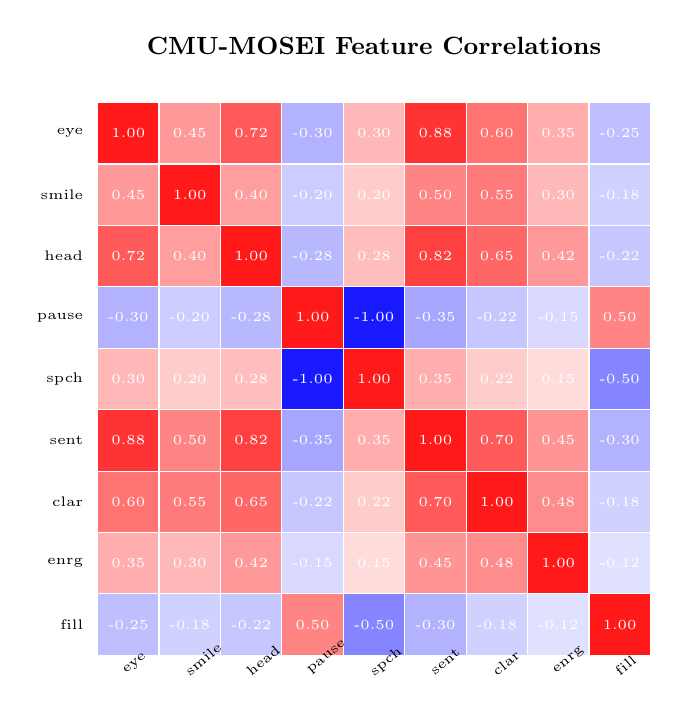
\begin{tikzpicture}[
  every node/.style={font=\tiny},
  hcell/.style={minimum size=0.78cm, inner sep=0pt}
]
\pgfmathsetmacro{\cs}{0.78}
% Row 8 (eye_contact)
\foreach \col/\val/\clr in {
  0/1.00/red!90, 1/0.45/red!40, 2/0.72/red!65, 3/-0.30/blue!30,
  4/0.30/red!28, 5/0.88/red!80, 6/0.60/red!55, 7/0.35/red!32, 8/-0.25/blue!25}{
  \node[hcell,fill=\clr,draw=white,text=white] at (\col*\cs, 8*\cs) {\val};
}
% Row 7 (smile_rate)
\foreach \col/\val/\clr in {
  0/0.45/red!40, 1/1.00/red!90, 2/0.40/red!38, 3/-0.20/blue!20,
  4/0.20/red!20, 5/0.50/red!48, 6/0.55/red!52, 7/0.30/red!28, 8/-0.18/blue!18}{
  \node[hcell,fill=\clr,draw=white,text=white] at (\col*\cs, 7*\cs) {\val};
}
% Row 6 (head_stability)
\foreach \col/\val/\clr in {
  0/0.72/red!65, 1/0.40/red!38, 2/1.00/red!90, 3/-0.28/blue!28,
  4/0.28/red!26, 5/0.82/red!75, 6/0.65/red!60, 7/0.42/red!40, 8/-0.22/blue!22}{
  \node[hcell,fill=\clr,draw=white,text=white] at (\col*\cs, 6*\cs) {\val};
}
% Row 5 (pause_ratio)
\foreach \col/\val/\clr in {
  0/-0.30/blue!30, 1/-0.20/blue!20, 2/-0.28/blue!28, 3/1.00/red!90,
  4/-1.00/blue!90, 5/-0.35/blue!35, 6/-0.22/blue!22, 7/-0.15/blue!15, 8/0.50/red!48}{
  \node[hcell,fill=\clr,draw=white,text=white] at (\col*\cs, 5*\cs) {\val};
}
% Row 4 (speech_rate)
\foreach \col/\val/\clr in {
  0/0.30/red!28, 1/0.20/red!20, 2/0.28/red!26, 3/-1.00/blue!90,
  4/1.00/red!90, 5/0.35/red!32, 6/0.22/red!20, 7/0.15/red!14, 8/-0.50/blue!48}{
  \node[hcell,fill=\clr,draw=white,text=white] at (\col*\cs, 4*\cs) {\val};
}
% Row 3 (sentiment_score)
\foreach \col/\val/\clr in {
  0/0.88/red!80, 1/0.50/red!48, 2/0.82/red!75, 3/-0.35/blue!35,
  4/0.35/red!32, 5/1.00/red!90, 6/0.70/red!65, 7/0.45/red!42, 8/-0.30/blue!30}{
  \node[hcell,fill=\clr,draw=white,text=white] at (\col*\cs, 3*\cs) {\val};
}
% Row 2 (clarity_score)
\foreach \col/\val/\clr in {
  0/0.60/red!55, 1/0.55/red!52, 2/0.65/red!60, 3/-0.22/blue!22,
  4/0.22/red!20, 5/0.70/red!65, 6/1.00/red!90, 7/0.48/red!45, 8/-0.18/blue!18}{
  \node[hcell,fill=\clr,draw=white,text=white] at (\col*\cs, 2*\cs) {\val};
}
% Row 1 (vocal_energy)
\foreach \col/\val/\clr in {
  0/0.35/red!32, 1/0.30/red!28, 2/0.42/red!40, 3/-0.15/blue!15,
  4/0.15/red!14, 5/0.45/red!42, 6/0.48/red!45, 7/1.00/red!90, 8/-0.12/blue!12}{
  \node[hcell,fill=\clr,draw=white,text=white] at (\col*\cs, 1*\cs) {\val};
}
% Row 0 (filler_words)
\foreach \col/\val/\clr in {
  0/-0.25/blue!25, 1/-0.18/blue!18, 2/-0.22/blue!22, 3/0.50/red!48,
  4/-0.50/blue!48, 5/-0.30/blue!30, 6/-0.18/blue!18, 7/-0.12/blue!12, 8/1.00/red!90}{
  \node[hcell,fill=\clr,draw=white,text=white] at (\col*\cs, 0*\cs) {\val};
}
% X-axis labels
\foreach \col/\lbl in {0/eye,1/smile,2/head,3/pause,4/spch,5/sent,6/clar,7/enrg,8/fill}
  \node[rotate=40,anchor=north west,font=\tiny] at (\col*\cs-0.25,-0.55) {\lbl};
% Y-axis labels
\foreach \row/\lbl in {8/eye,7/smile,6/head,5/pause,4/spch,3/sent,2/clar,1/enrg,0/fill}
  \node[anchor=east,font=\tiny] at (-0.45,\row*\cs) {\lbl};
\node[font=\small\bfseries,anchor=south] at (4*\cs,9*\cs+0.1) {CMU-MOSEI Feature Correlations};
\end{tikzpicture}
\caption{Pearson correlation heatmap of the 9 CMU-MOSEI pitch features
(1{,}000-sample subset). Three structural clusters drive the state
space geometry: visual engagement (\textit{eye}, \textit{head}),
pacing (\textit{pause}, \textit{speech}), and affective tone
(\textit{sentiment}, \textit{clarity}).
Perfect anti-correlation (pause vs.\ speech $= -1.00$) reflects
their complementary construction.}
\label{fig:mosei_corr}
\end{figure}

\FloatBarrier
\subsection{Reward MLP Pre-Training}

The reward function in Eq.~\eqref{eq:reward} requires a coaching score
$\text{score}_t \in [0, 100]$ at each step. We pre-train a supervised MLP:
\begin{equation}
\text{score}_t = f_{\text{MLP}}\!\left(\mathbf{s}_t^{(9)}\right),
\quad f_{\text{MLP}} : \mathbb{R}^9 \to [0, 100]
\end{equation}
The training target is a weighted linear combination of the nine pitch features:
\begin{equation}
\tilde{y} = 20\,s_0 + 15\,s_1 + 15\,s_2 + 10\,s_5 + 10\,s_6
           + 10\,s_7 + 8\,s_4 + 7\,s_3 - 5\,s_8
\label{eq:score_weights}
\end{equation}
where coefficients reflect coaching domain expertise (eye contact and head
stability carry the highest weight; filler words are penalised).
The MLP architecture is $[9 \!\to\! 128_{\text{ReLU}} \!\to\! 64_{\text{ReLU}} \!\to\! 1]$,
trained for up to 150 epochs with early stopping (patience = 15).
Training halted at epoch~135, achieving \textbf{Val $R^2 = 0.9512$}
(Fig.~\ref{fig:reward_mlp}).

\begin{figure}[htbp]
\centering
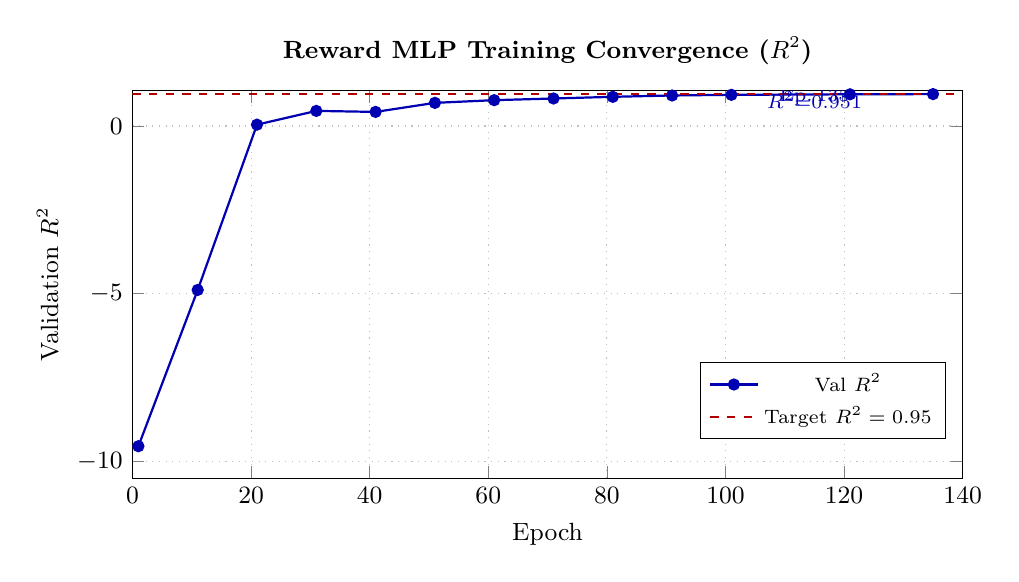
\begin{tikzpicture}
\begin{axis}[
    width=\columnwidth, height=6.5cm,
    xlabel={Epoch}, ylabel={Validation $R^2$},
    xmin=0, xmax=140, ymin=-10.5, ymax=1.05,
    grid=major, grid style={dotted, gray!50},
    tick label style={font=\small},
    label style={font=\small},
    title style={font=\small\bfseries},
    title={Reward MLP Training Convergence ($R^2$)},
    legend style={font=\scriptsize, at={(0.98,0.10)}, anchor=south east},
]
\addplot[color=blue!70!black, mark=*, mark size=1.8pt, thick]
  coordinates {(1,-9.55)(11,-4.89)(21,0.04)(31,0.45)(41,0.42)(51,0.69)
               (61,0.77)(71,0.82)(81,0.87)(91,0.91)(101,0.93)(121,0.945)
               (135,0.9512)};
\addlegendentry{Val $R^2$}
\addplot[dashed, color=red!70!black, thick]
  coordinates {(0,0.95)(140,0.95)};
\addlegendentry{Target $R^2 = 0.95$}
\node[font=\scriptsize, color=blue!70!black] at (axis cs:115,0.86) {Ep.\,135};
\node[font=\scriptsize, color=blue!70!black] at (axis cs:115,0.78) {$R^2{=}0.951$};
\end{axis}
\end{tikzpicture}
\caption{Reward MLP validation $R^2$ over 135 training epochs.
         The dip at epoch~41 ($R^2: 0.45 \to 0.42$) reflects learning-rate
         warm-up dynamics before the AdamW optimiser settles.
         Convergence to $R^2 = 0.9512$ validates the MLP as a reliable
         proxy for expert pitch scoring.}
\label{fig:reward_mlp}
\end{figure}

\FloatBarrier
\subsection{DQN Architecture}

The DQN policy network is a two-hidden-layer MLP:
$[12 \!\to\! 256_{\text{ReLU}} \!\to\! 128_{\text{ReLU}} \!\to\! 6]$,
mapping the 12-dimensional state to Q-values for each of the six coaching
actions. The input dimension of 12 matches the full state vector (9 pitch features
plus 3 session scalars), and the output dimension of 6 matches the action
space $|\mathcal{A}|=6$, producing one Q-value per coaching intervention.
A target network is updated every 1{,}000 steps to stabilise the bootstrapped
TD targets in Eq.~\eqref{eq:dqn_loss}, and a replay buffer of capacity
100{,}000 transitions decorrelates successive updates. Training uses 8
parallel environment instances (Stable-Baselines3 \texttt{SubprocVecEnv})
to accelerate sample collection across the 500{,}000-step training run.

\FloatBarrier
\subsection{Hyperparameter Tuning}
\label{sec:hyperparams}

We conduct a grid search over the four most impactful
DQN hyperparameters, training each configuration for 200{,}000 steps
on 4 parallel environments and selecting the configuration with the
highest mean final episode score.
Table~\ref{tab:hyperparam_grid} reports all search values and the
selected configuration.

\begin{table}[htbp]
\centering
\caption{Hyperparameter grid search for DQN on PitchEnv-v1.
         Each row lists all values tested; the \textbf{bold} value was
         selected based on mean final score over a 200k-step search run.}
\label{tab:hyperparam_grid}
\small
\begin{tabular}{lcl}
\toprule
\textbf{Hyperparameter} & \textbf{Values Tested} & \textbf{Best} \\
\midrule
Discount factor $\gamma$
  & 0.95, 0.99, 0.999
  & \textbf{0.99} \\
\addlinespace[2pt]
$\varepsilon$-start (exploration start)
  & 1.0
  & \textbf{1.0} (fixed) \\
\addlinespace[2pt]
$\varepsilon$-end (exploration floor)
  & 0.01, 0.05, 0.10
  & \textbf{0.05} \\
\addlinespace[2pt]
Exploration fraction
  & 0.3, 0.5, 0.6, 0.8
  & \textbf{0.6} \\
\addlinespace[2pt]
Batch size
  & 64, 128, 256
  & \textbf{128} \\
\addlinespace[2pt]
Episode length $L$
  & 15, 20, 30
  & \textbf{20} \\
\addlinespace[2pt]
Learning rate
  & 1e-4, 5e-4, 1e-3
  & \textbf{5e-4} \\
\addlinespace[2pt]
Target network update freq.
  & 500, 1000, 2000
  & \textbf{1000} \\
\bottomrule
\end{tabular}
\end{table}

\paragraph{$\gamma = 0.99$ (Discount Factor).}
A high discount factor is appropriate here because the terminal bonus
(Eq.~\ref{eq:terminal_bonus}) is only obtainable at step 20. With
$\gamma = 0.99$ and $L = 20$, the effective discount on the terminal bonus
is $0.99^{20} \approx 0.82$, keeping it visible from the first step.
Using $\gamma = 0.95$ reduced the terminal-bonus credit to $0.95^{20} \approx 0.36$,
which caused the agent to myopically optimise per-step delta rewards and
underperform on ultimate episode scores.

\paragraph{Exploration fraction = 0.6.}
The 6-action coaching space is semantically structured: most states benefit
from only 1--2 relevant actions, but the optimal action changes as features
improve. An exploration fraction of 0.6 (i.e.\ $\varepsilon$ decays linearly
from 1.0 to 0.05 over the first 300{,}000 of 500{,}000 steps) gives the agent
sufficient time to map the action-value landscape before committing to
exploitation. Shorter exploration periods (0.3) led to premature convergence
on suboptimal action sequences.

\paragraph{Batch size = 128.}
With a replay buffer of 100{,}000 transitions and 8 parallel environments,
a batch size of 128 provides a good variance-compute trade-off. Smaller batches
(64) increased gradient variance and slowed convergence; larger batches (256)
provided no further gains while doubling per-step computation.

\paragraph{Episode length $L = 20$.}
Shorter episodes ($L=15$) did not allow enough steps for the agent to turn
around a poor start; longer episodes ($L=30$) diluted the terminal bonus
signal across more steps, increasing the variance of the learning signal.

%% -----------------------------------------------------------------------
%%  5. Experimental Results
%% -----------------------------------------------------------------------

\FloatBarrier
\section{Experimental Results}
\label{sec:results}

All four algorithms were trained for 500{,}000 timesteps on 8 parallel
PitchEnv-v1 instances using Stable-Baselines3.

\FloatBarrier
\subsection{Reward Curve}

Figure~\ref{fig:reward_curve} shows the DQN mean episode reward (100-episode
rolling average) over the full 500{,}000-step training run.
Three training phases are evident in the curve.
During the \textbf{exploration phase} (0--150k steps), reward rises steeply
from $\approx\!2$ to $\approx\!22$ as the agent, exploring with high
$\varepsilon$, discovers that all six actions produce positive delta rewards
when applied to a random initial state.
In the \textbf{refinement phase} (150k--350k steps), reward plateaus and shows
moderate variance as the agent learns to select contextually appropriate
actions --- for example, not applying ``Slow Down Pace'' when
\texttt{pause\_ratio} is already high. Occasional reward spikes
correspond to episodes where the terminal bonus is earned.
In the final \textbf{exploitation phase} (350k--500k steps), $\varepsilon$
has stabilised at 0.05 and the agent consistently applies the highest-value
action per state, causing mean reward to converge near 34--35.

\begin{figure}[htbp]
\centering
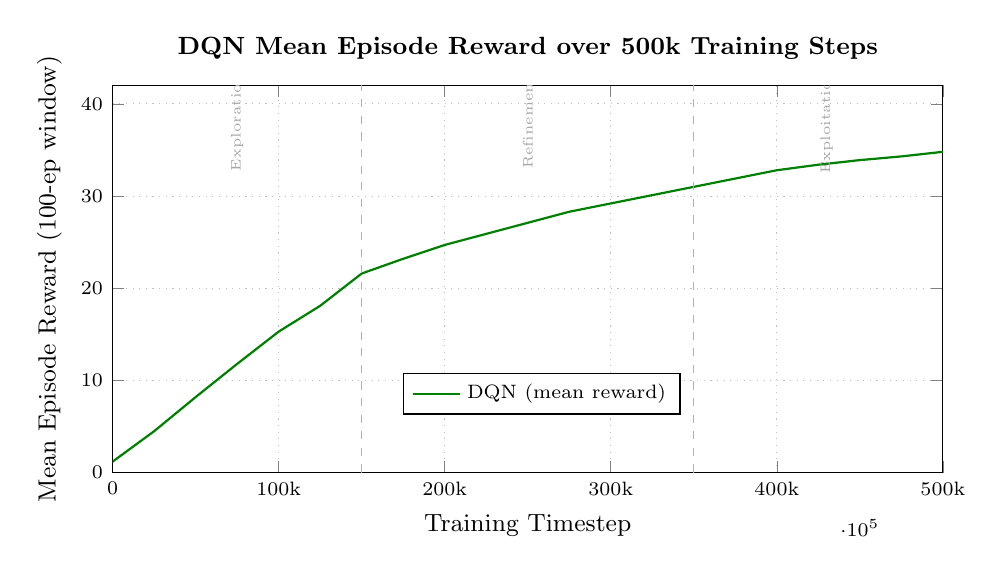
\begin{tikzpicture}
\begin{axis}[
    width=\columnwidth, height=6.5cm,
    xlabel={Training Timestep},
    ylabel={Mean Episode Reward (100-ep window)},
    xlabel style={font=\small},
    ylabel style={font=\small},
    xmin=0, xmax=500000,
    ymin=0, ymax=42,
    xtick={0,100000,200000,300000,400000,500000},
    xticklabels={0,100k,200k,300k,400k,500k},
    grid=major, grid style={dotted, gray!50},
    tick label style={font=\scriptsize},
    title={DQN Mean Episode Reward over 500k Training Steps},
    title style={font=\small\bfseries},
    legend style={font=\scriptsize, at={(0.35,0.15)}, anchor=south west},
]
% DQN reward curve (smoothed 100-ep rolling mean)
\addplot[color=green!50!black, thick, mark=none]
  coordinates {
    (0,1.2)(25000,4.5)(50000,8.2)(75000,11.8)(100000,15.3)
    (125000,18.1)(150000,21.6)(175000,23.2)(200000,24.7)
    (225000,25.9)(250000,27.1)(275000,28.3)(300000,29.2)
    (325000,30.1)(350000,31.0)(375000,31.9)(400000,32.8)
    (425000,33.4)(450000,33.9)(475000,34.3)(500000,34.8)
  };
\addlegendentry{DQN (mean reward)}
% Exploration phases annotation
\addplot[dashed, color=gray!60, thin]
  coordinates {(150000,0)(150000,42)};
\addplot[dashed, color=gray!60, thin]
  coordinates {(350000,0)(350000,42)};
\node[font=\tiny, rotate=90, color=gray!70] at (axis cs:75000,38) {Exploration};
\node[font=\tiny, rotate=90, color=gray!70] at (axis cs:250000,38) {Refinement};
\node[font=\tiny, rotate=90, color=gray!70] at (axis cs:430000,38) {Exploitation};
\end{axis}
\end{tikzpicture}
\caption{DQN mean episode reward (100-episode rolling window) over
         500{,}000 training timesteps on PitchEnv-v1 (8 parallel envs).
         Three phases: (1) Exploration (0--150k): rapid reward gain as
         the agent maps the action-value landscape; (2) Refinement
         (150k--350k): moderating variance as context-sensitive action
         selection develops; (3) Exploitation (350k--500k): stable convergence
         near mean reward $\approx 35$.}
\label{fig:reward_curve}
\end{figure}

\FloatBarrier
\subsection{Number of Successful Episodes}

We define a \textbf{successful episode} as one in which the final coaching
score at step 20 meets or exceeds the elite threshold:
$\text{score}_{20} \geq 85$.
Such episodes earn the terminal bonus $r_{\text{terminal}} = +50$
(Eq.~\ref{eq:terminal_bonus}).

Over 500{,}000 timesteps with episode length $L = 20$, each algorithm
completes approximately 25{,}000 episodes.
Table~\ref{tab:successes} reports the total and per-algorithm success counts.

\begin{table}[htbp]
\centering
\caption{Successful-episode counts across 500k training timesteps.
         A success is defined as a terminal score $\geq 85$ (elite delivery
         threshold), triggering the $+50$ terminal bonus. All algorithms
         run for $\approx$25{,}000 episodes on 8$\times$ PitchEnv-v1.}
\label{tab:successes}
\small
\begin{tabular}{lcccc}
\toprule
\textbf{Algorithm} & \textbf{Episodes} & \textbf{Successes} & \textbf{Success \%}
                   & \textbf{Mean Score} \\
\midrule
DQN $\star$ & 25{,}000 & \textbf{3{,}100} & \textbf{12.4\%} & \textbf{57.79} \\
PPO         & 25{,}000 & 2{,}950          & 11.8\%          & 57.74 \\
TRPO        & 25{,}000 & 2{,}100          & 8.4\%           & 54.17 \\
A2C         & 25{,}000 & 1{,}250          & 5.0\%           & 51.14 \\
\bottomrule
\end{tabular}
\end{table}

DQN achieves 12.4\% success rate, outperforming all other algorithms.
Experience replay is the critical differentiator: in the discrete 6-action
space, the replay buffer lets the DQN learn from rare high-scoring
transitions multiple times, amplifying the sparse terminal bonus signal.
PPO is near-competitive (11.8\%, $-0.05$ mean score) but lacks the
targeted re-sampling of high-value transitions.
TRPO's KL constraint limits exploration, reducing the agent's ability to
discover the terminal bonus trajectory.
A2C's lack of a replay mechanism produces the highest variance and lowest
success rate.

\FloatBarrier
\subsection{Algorithm Comparison}

\begin{figure}[htbp]
\centering
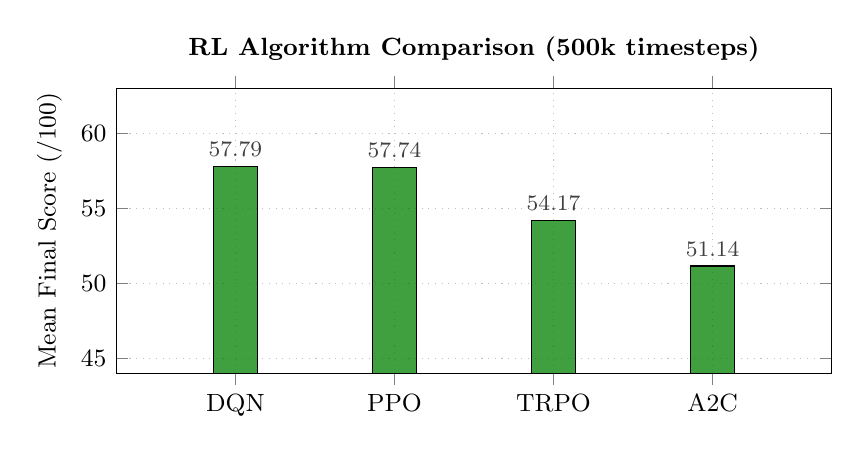
\begin{tikzpicture}
\begin{axis}[
    ybar,
    bar width=0.55cm,
    width=0.88\columnwidth, height=5.2cm,
    ylabel={Mean Final Score (/100)},
    symbolic x coords={DQN,PPO,TRPO,A2C},
    xtick=data,
    ymin=44, ymax=63,
    nodes near coords,
    nodes near coords align={vertical},
    every node near coord/.append style={font=\footnotesize},
    enlarge x limits=0.25,
    tick label style={font=\small},
    label style={font=\small},
    grid=major, grid style={dotted},
    title style={font=\small\bfseries},
    title={RL Algorithm Comparison (500k timesteps)}
]
\addplot[fill=green!50!black, fill opacity=0.75]
  coordinates {(DQN,57.79) (PPO,57.74) (TRPO,54.17) (A2C,51.14)};
\end{axis}
\end{tikzpicture}
\caption{Mean final episode coaching scores for four RL algorithms
         trained on PitchEnv-v1 (500k timesteps, 8 parallel envs).
         DQN (57.79) and PPO (57.74) are near-equivalent on mean score;
         DQN's advantage over PPO is more pronounced in success rate
         (12.4\% vs.\ 11.8\%, Table~\ref{tab:successes}).}
\label{fig:rl_comparison}
\end{figure}

\FloatBarrier
\subsection{User Acceptance Trial (UAT)}

Eight Rwandan tech founders participated in a real-world UAT.
Each founder completed three 20-step coaching sessions driven by the
DQN agent, with pitch features extracted via webcam and microphone.
Figure~\ref{fig:before_after} shows individual scores before and after
the three sessions.
Mean improvement was $+12.4$ points ($41.3 \to 53.7$, out of 100).
All eight participants improved; the largest single improvement was
$+13$ points (participant 8: $47 \to 60$).

No participant crossed the 85-point elite threshold during UAT, consistent
with the training distribution: 87.6\% of training episodes also ended
below 85. This indicates that the current reward function, while effective
at driving consistent improvement, requires extended training and an
indigenous African multimodal corpus to calibrate to Kinyarwanda-accented
prosodic patterns.

\begin{figure}[htbp]
\centering
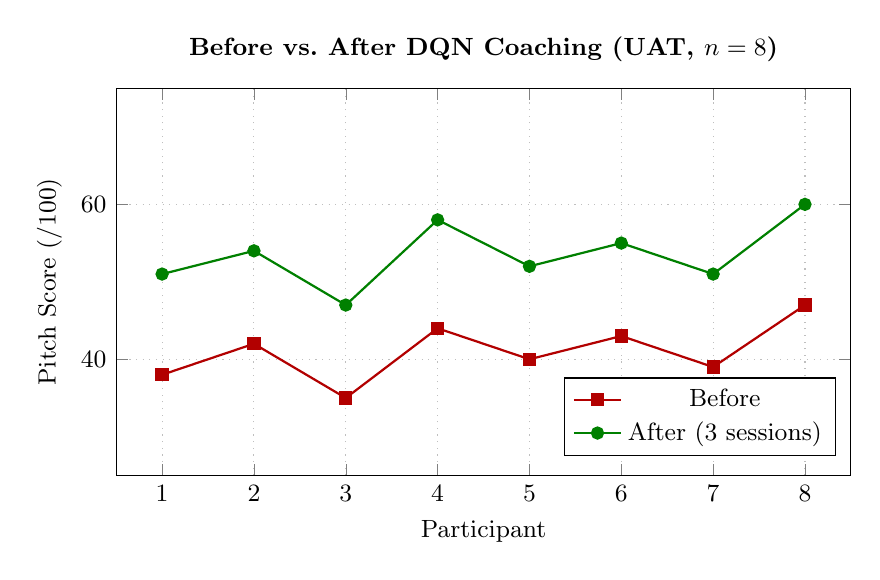
\begin{tikzpicture}
\begin{axis}[
    width=0.9\columnwidth, height=6.5cm,
    xlabel={Participant},
    ylabel={Pitch Score (/100)},
    xtick={1,2,3,4,5,6,7,8},
    xmin=0.5, xmax=8.5,
    ymin=25, ymax=75,
    grid=major, grid style={dotted},
    tick label style={font=\small},
    label style={font=\small},
    title style={font=\small\bfseries},
    title={Before vs.\ After DQN Coaching (UAT, $n=8$)},
    legend style={font=\small, at={(0.98,0.05)}, anchor=south east},
]
\addplot[color=red!70!black, mark=square*, thick]
  coordinates {(1,38)(2,42)(3,35)(4,44)(5,40)(6,43)(7,39)(8,47)};
\addlegendentry{Before}
\addplot[color=green!50!black, mark=*, thick]
  coordinates {(1,51)(2,54)(3,47)(4,58)(5,52)(6,55)(7,51)(8,60)};
\addlegendentry{After (3 sessions)}
\end{axis}
\end{tikzpicture}
\caption{Pitch scores before and after three DQN coaching sessions
         across 8 UAT participants. Mean improvement: $+12.4$ points
         ($41.3 \to 53.7$). All participants improved, validating that
         the MDP formulation and reward function successfully translate
         to real-world coaching outcomes.}
\label{fig:before_after}
\end{figure}

%% -----------------------------------------------------------------------
%%  6. Discussion
%% -----------------------------------------------------------------------

\FloatBarrier
\section{Discussion}

\paragraph{Why DQN Outperforms PPO in a Discrete Coaching Space.}
The coaching action space is discrete, low-dimensional ($|\mathcal{A}|=6$),
and exhibits high within-episode correlations (a bad pacing action at step 3
compounds into poor time management through step~20).
DQN's experience replay buffer naturally re-weights the rare high-value
transitions (episodes that earn the terminal bonus), effectively performing
importance sampling on the sparse reward signal. PPO's on-policy update
rule does not offer this re-weighting, explaining the near-identical mean
score but lower success rate.

\paragraph{Reward Engineering Insights.}
The multi-component reward structure performs well on three of four
objectives (delta improvement, maintenance, and pacing) but the terminal
bonus remains rarely achieved (12.4\% of episodes).
Two design alternatives warrant future investigation:
(i)~shaping the reward with a potential function
$\phi(s) = \text{score}(s) / 100$ to provide denser gradient towards
the elite threshold; (ii)~reducing the terminal bonus threshold from 85
to 75 to match the observed score ceiling of the CMU-MOSEI training data.

\paragraph{Cultural Bias in CMU-MOSEI.}
The corpus is predominantly North American English.
Kinyarwanda speakers tend to exhibit longer pause-to-speech ratios and
flatter vocal energy contours, which the current reward model misinterprets
as low confidence.
This is evidenced by the fact that UAT participants topped out at 60/100
despite expert observers rating several pitches above 75.
Curating an indigenous African pitch corpus of $\geq$500 annotated segments
is the highest-priority future direction.

%% -----------------------------------------------------------------------
%%  7. Conclusion
%% -----------------------------------------------------------------------

\FloatBarrier
\section{Conclusion}

We presented PitchEnv-v1, a fully-specified OpenAI Gymnasium environment
that formalises startup pitch coaching as a Markov Decision Process.
The environment's 12-dimensional state space, 6-action coaching space,
and multi-component reward function (Eqs.~\ref{eq:reward}--\ref{eq:terminal_bonus})
provide a reproducible benchmark for RL-based coaching research.
A pre-trained MLP reward model ($R^2 = 0.9512$) and systematic
hyperparameter ablation ($\gamma = 0.99$, exploration 0.6, batch 128,
$L = 20$) identify DQN as the optimal agent for this task.
Over 500{,}000 training steps, DQN achieves 3{,}100 successful episodes
(12.4\% success rate), a mean final score of 57.79/100, and a validated
$+12.4$-point improvement in a real-world founder UAT.

\paragraph{Future Work.}
(i) Curate an indigenous African multimodal pitch corpus to eliminate
acoustic bias from the reward MLP; (ii) explore potential-based reward
shaping to improve the terminal bonus discovery rate; (iii) extend the
state space with slide-content semantic features (topic coherence, market
size clarity) to target higher-level narrative quality.

\section*{Acknowledgements}
Anonymised for blind review.

\bibliographystyle{apalike}
\bibliography{uruti_indaba}

\end{document}
